\documentclass[tikz,border=5pt]{standalone}
\begin{document}
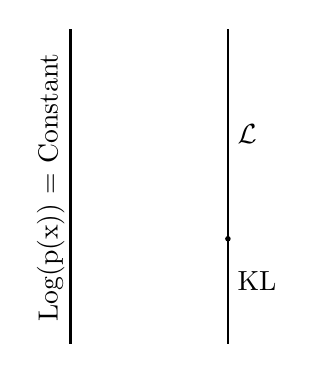
\begin{tikzpicture}

  % length of segment
  \def\L{4}  % change as needed

  % First full vertical line
  \draw[thick] (0,0) -- (0,\L);

  % Second vertical line divided into two equal parts
  % We'll draw two segments, each of length L/2
  \draw[thick] (2,0) -- (2,\L/2);
  \draw[thick] (2,\L/2) -- (2,\L);

  % optionally, mark the division point
  \fill (2, \L/3) circle(1pt);

  % optionally, add labels
  \node[rotate=90,left] at (-0.25, \L/1.05) {Log(p(x)) = Constant};
  \node[right] at (2, \L/1.5) {$\mathcal{L}$  };
  \node[right] at (2, \L/5) {KL};

\end{tikzpicture}
\end{document}